\documentclass[a4paper,dvipsnames,headsepline,8pt,twocolumn]{scrartcl}
\usepackage[utf8]{inputenc}
% \usepackage[margin=1in]{geometry}
\usepackage{graphicx}    % For including images
\usepackage{xcolor}      % For colored text (e.g., to highlight commands)
\definecolor{skyblue1}{RGB}{114,159,207}
\definecolor{plum1}{RGB}{173,127,168}
\definecolor{chameleon1}{RGB}{78,154,6}
\usepackage{hyperref}    % For hyperlinks
\hypersetup{
    colorlinks=true,
    linkcolor=MidnightBlue,
    filecolor=magenta,      
    urlcolor=MidnightBlue,
    citecolor=plum1,
    pdftitle={GA3 training},
    % pdfpagemode=FullScreen,
    }
\usepackage{menukeys}   % forkeys and menu
% \renewmenumacro{\menu}[>]{shadowedroundedkeys}
\renewmenumacro{\directory}[/]{pathswithfolder}
\usepackage{listings}   % for code
\usepackage{siunitx}
\usepackage{lmodern}    % the font
\renewcommand{\familydefault}{\sfdefault}  % sans serif fonts
\usepackage{booktabs}   % nicer table
\usepackage{fourier}    % warning symbol
\pagestyle{headings}     % use srartcl headings style
\usepackage{tikz}
\usepackage{pgfplots}
\usetikzlibrary{decorations.pathmorphing}
\usepgfplotslibrary{fillbetween}
\pgfplotsset{compat=1.18} 
\usepackage{enotez}      % create end notes with the solutions
\setenotez{backref=true}
\usepackage{pixels}
\usepackage{biblatex}
\bibliography{refs.bib}

\title{Nikon NIS-Elements\\ General Analysis 3}
\author{Light microscopy facility - MRC LMB}
\date{June 2025}

\begin{document}


\maketitle

\paragraph{Objectives}
By the end of this workshop, participant will be able to:
\begin{itemize}
\item Given acquired microscope image data, create a GA3 recipe to accurately quantify image content.
\item From generated results, store data as both table and binary files, following best practices.
\item Given a newly created GA3 recipe, apply it to batch process a given set of images independently.
\end{itemize}

\paragraph{Contributors}
Nick Barry, Jérôme Boulanger, Ben Sutcliffe, Dina Ratsimandresy

\tableofcontents % % \newpage
\section{Introduction}

This course has been tested on NIS Elements version 5.42.

\subsection{General interface}


\paragraph{Preliminary steps}
Once the GA3 module opened, other windows cannot be opened, therefore
\begin{itemize}
    \item you will need to open the image you want to work with first,
    \item it is convenient to open the LUT tools first (\keys{\ctrl+\Alt+L}),
    \item opening the help  can also be useful.
\end{itemize}
To access the GA3 interface, you can either:
\begin{itemize}
    \item use the menu \menu{Image>New GA3 recipe\dots},
    \item use the menu \menu{Image>Analysis Explorer\dots} to open the analysis exporter and then click on \menu{Create New},
    \item right-click on the background of the interface, select \menu{Analysis Controls>Analysis Explorer} to open the analysis explorer and then click on \menu{Create New}.
\end{itemize}

\paragraph{Loading and saving recipes}

\begin{itemize}
    \item Use \menu{Save} or \menu{Save As} to save the recipe in the local database. It will be then listed in the Analysis Explorer.
    \item Use your name as a prefix so that we can contact you if the database needs to be cleared.
    \item Use \menu{Export} to export the recipe in a folder of your choice. This recipe can then be reloaded on another computer. It is good practice to have a copy of the recipes in that way.
    \item Use \menu{Import} to reload an exported recipe. 
\end{itemize}

\paragraph{Recipes}
\begin{figure*}
    \centering \small
    \begin{tikzpicture}
        \node at (0,0) {\includegraphics[width=0.75\textwidth]{artwork/simple-workflow.png}};
        % \draw[gray,very thin,step=1] (-5,-1) grid (5,1);
        \node (a) at (-5,-0.5){color};
        \node (b) at (-2.5,-0.5) {action};
        \node (c) at (0,-0.5) {binary};
        \node (d) at (5,-0.5) {table};
        \draw[->] (a) -| ++(1,0.4); 
        \draw[->] (b) -| ++(1,0.4); 
        \draw[->] (c) -| ++(1,0.4); 
        \draw[->] (d) -| ++(1,0.4); 
    \end{tikzpicture}
    \caption{A simple workflow with three kinds of nodes.}
    \label{fig:nodes}
\end{figure*}

Recipes describe a workflow as a graph. The graph is composed of 4 types of nodes (See Fig.~\ref{fig:nodes}):
\begin{enumerate}\setlength\itemsep{0em}
    \item color: original or processed grayscale images
    \item action: processing steps on images, binary or tables
    \item binary: masks and labels
    \item results: tables with measurement results 
\end{enumerate}

To add an action, drag the new element to the previous one to automatically create a connection and keep the elements organized. You can also use \keys{\shift} and left click circling the elements to select them. Finally, a group of elements can be combined to create a function.

\paragraph{Storing results}

Saving of channels and binary layers can be enabled case by case using a right click on the layer and selecting ``store this result'' or ``do not store this result''.


\subsection{Tips}
\begin{itemize}
    \item Use \keys{\Alt+\arrowkeyup} / \keys{\Alt+\arrowkeydown}  to increase / decrease the opacity of the binaries.
    \item To look for a module, use the search bar at the top.
    \item Right-click on the image and find image information for pixel to micron conversion.
    \item Click on the question mark on each operation (top left) for more information if needed.
\end{itemize}

\subsection{Basic image processing concepts}

\paragraph{Image} An image is any array (table) of regularly sampled intensity value. The values can range between $0$ and $2^8 = 255$ for 8-bit images or between $0$ and $2^{16}=65635$ for 16 bit images. Figure~\ref{fig:median} displays an image as graylevel and intensities values.

\paragraph{Threshold} Threshold is the simplest form of image segmentation. At each location of the image, a decision is taken to classify this point as foreground or background. In GA3, thresholds are followed by other operations such as smoothing, cleaning, connected component labelling, size filtering,\dots Here threshold are defined by a range with a minimum and maximum intensity. In fluorescence microscopy, we often want the minimum of this range to be more than 0 and the maximum untouched.

\paragraph{Median filter} The median filter is creating a new image where each pixel is computed as the median value of the pixels in a neighborhood of this pixel (See Figure~\ref{fig:median}). The median filter is a good approach for reducing the noise whilst preserving the edges of the image.

\begin{figure}[ht]\centering
    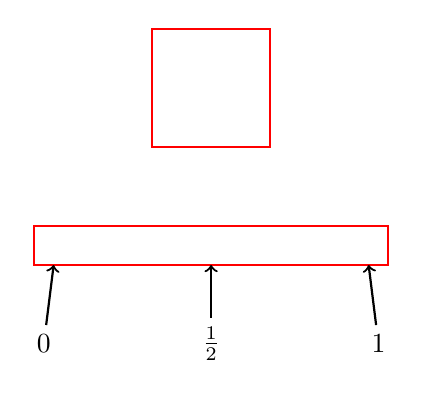
\begin{tikzpicture}[scale=0.5]
    \begin{scope}
        \def\pixels{{10,5,6,2,9},{8,5,2,4,8},{4,8,6,3,1},{2,9,7,10,3},{3,6,6,2,9}}
        \showpixelsvalue{\pixels}{0}{10}
        \draw[red,thick] (2,2) rectangle +(3,3);
    \end{scope}
    \begin{scope}[yshift=-2cm,xshift=-2cm]
        \def\pixels{{2,3,4,5,6,7,8,9,10}} 
        \showpixelsvalue{\pixels}{0}{10}
        \draw[red,thick] (1,1) rectangle +(9,1);
        \draw (1.25,-1) node {$0$} edge[->,thick] (1.5,1);
        \draw (5.5,-1) node {$\frac{1}{2}$} edge[->,thick] (5.5,1);
        \draw (9.75,-1) node {$1$} edge[->,thick] (9.5,1);
    \end{scope}
    \end{tikzpicture}
    \caption{Values in a $3 \times 3$ neighborhood are ordered to define a median (rank 1/2)
    filter. The intensity corresponding to the median value is stored in a new image.}
    \label{fig:median}
\end{figure}

\paragraph{Morphological erosion and dilation} Erosion and dilation are morphological operations on the image. They can be expressed both for binary and grayscale images are the minimum and respectively maximum of the pixels in a neighborhood depicted in red in Figure.~\ref{fig:median}, \textit{i.e.} ranks 0 and 1. In practice, this neighborhood could have various shapes and also have a different weight. Formally, the erosion of a and image $f$ at each pixel $x$ by a structuring element with weights $b$ defined as $(f \oplus b)(x) = \inf_{y} f(x+y) - b(y)$ and the dilation as $(f \ominus b)(x) = \sup_{y} f(y) + b(x-y)$. The result is an image with smaller, and respectively bigger, bright areas enabling to expand and shrink region.

\paragraph{Morphological opening and closing} Opening and closing are also morphological operations resulting of the combination an erosion followed by a dilation, and respectively, the dilation followed by an erosion. Formally, the opening is defined as $f \circ b  = (f \ominus b) \oplus b$ and the closing is defined as $f \bullet  b  = (f \oplus b) \ominus b$.

\paragraph{Rolling ball} Rolling ball~\cite{sternberg1983} is used for correcting shading and non-even background. It works by subtracting a background image estimated by a morphological opening the image using a structuring element which has radially decaying weights (the ball).

\begin{figure}[ht]\centering
    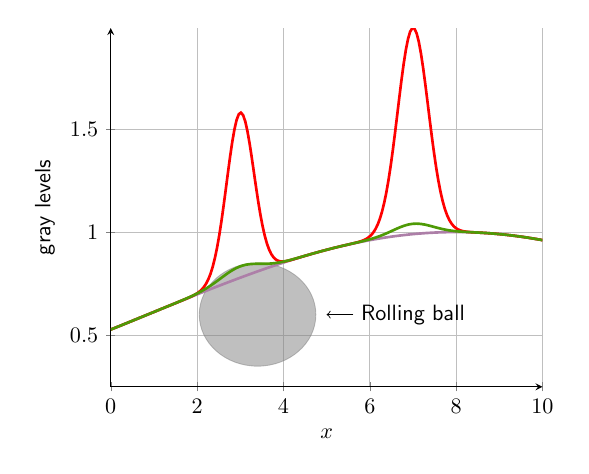
\begin{tikzpicture}[scale=0.8]
        \begin{axis}[
            axis lines=left, 
            xlabel={$x$},
            ylabel={gray levels},
            domain=0:10,
            grid=major,
            samples=200,
            ymin=0.25,
        ]
        \draw [gray,fill,opacity=0.5] (3.4,0.6) ellipse [x radius=1.35, y radius=0.25]; 
        \node (c) at (7,0.6){Rolling ball};
        \addplot[plum1,very thick] {exp(-(x-8)^2 / 100)};
        \addplot[red,very thick] {0.8*exp(-(x-3)^2 / 0.2)+exp(-(x-7)^2 / 0.25)+exp(-(x-8)^2 / 100)};
        \addplot[chameleon1,very thick] {0.055*exp(-(x-3)^2 / 0.4)+0.05*exp(-(x-7)^2 / 0.4)+exp(-(x-8)^2 / 100)};
        \draw[->] (c) -- (5,0.6);
        \end{axis} 
    \end{tikzpicture}
    \caption{Illustration of the rolling ball.}
    \label{fig:algorithm}
\end{figure}

\begin{figure}[ht]\centering
    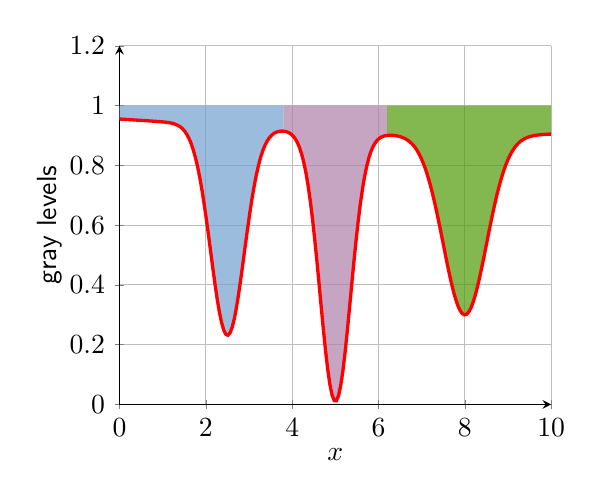
\begin{tikzpicture}[scale=0.8]
        \begin{axis}[
            axis lines=left, 
            xlabel={$x$},
            ylabel={gray levels},
            domain=0:10,
            grid=major,
            samples=200,
            ymin=0.0,
            ymax=1.2,
        ]
        \addplot[red,very thick,name path=A] {1-(0.7*exp(-(x-2.5)^2 / 0.3)+0.9*exp(-(x-5)^2 / 0.25)+0.6*exp(-(x-8)^2 / 0.5))-0.1*exp(-(x-8)^2 / 80)};
        \addplot+[draw=none, no markers, name path=B] {1}; 
        \addplot[skyblue1,opacity=0.7] fill between[
            of=A and B,
            soft clip={domain=0:3.8}
        ];
        \addplot[plum1,opacity=0.7] fill between[
            of=A and B,
            soft clip={domain=3.8:6.2}
        ];        
        \addplot[chameleon1,opacity=0.7] fill between[
            of=A and B,
            soft clip={domain=6.2:10}
        ];
        
        \end{axis} 
    \end{tikzpicture}
    \caption{Illustration of the watershed algorithms of the digital elevation model (DEM) with 3 flooded depressions. The seeds or sources are the local minima of the DEM.}
    \label{fig:watershed}
\end{figure}



\paragraph{Watershed} The watershed algorithm associate to seed regions pixels in the image in the order of a priority map. It can also be interpreted as flooding a landscape or digital elevation model (DEM) (see Figure~\ref{fig:watershed}). In practice, several algorithms can be considered for implementing a watershed. One of them is called ``priority-flood''~\cite{barnes2014} where starting from seeds, each neighboring pixels (e.g. $3 \times 3$) are added to a queue by order of priority given by a priority map (minimum elevation of the landscape). The queue keeps track of the priority value, the location and the label of the basin. Seeds can be defined as local minima of the landscape function. At each iteration, the highest priority element is popped out of the queue, if not already labeled the pixel if attributed the label of the current basin and its neighbors added to the queue.

\paragraph{Pearson correlation coefficient} The Pearson correlation coefficient (PCC)~\cite{pcc} is a statistical tool used to measure the linear correlation between two signal indicating the potential co-localization of two labelled molecules population. If we have the pair of red and green intensities $(r_i,g_i)$ at each location $i$ in the image, the PCC is defined as 
$$\mathrm{pcc} = \frac{\sum_i(r_i-\bar{r})(g_i-\bar{g})}{\sum_i(r_i-\bar{r})^2 \sum_i(g_i-\bar{g})^2}$$ 
with the means $\bar{r} = n^{-1}\sum_i r_i$ and $\bar{g} = n^{-1}\sum_i g_i$. The value of the PCC ranges from -1 to 1 where a value of 1 indicates a linear correlation.

\paragraph{Table join} To combine measurements from two tables, we can use a ``join''~\cite{join} which will find the  rows base sharing a common reference index. The ``inner join'' operation will include only the matching row in both tables (See Figure~\ref{fig:join}). Manipulating table can replace logical operation on binary masks when combined with object parenting. In the simpler case where table have the same corresponding rows in the same order, tables can be simply collated with each other.

\begin{figure}[ht]\centering
    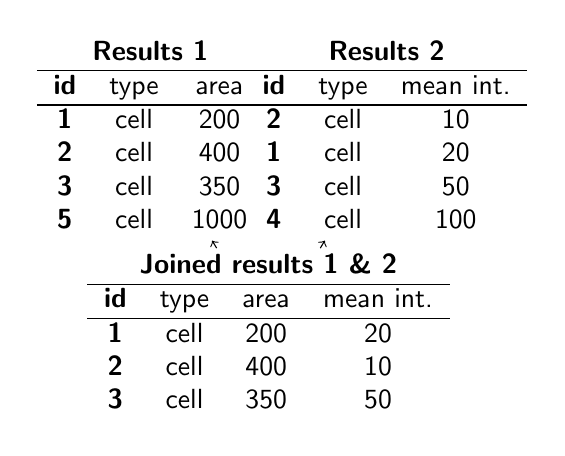
\begin{tikzpicture}
        \node (A) at (0,2.5) {
            \begin{tabular}{>{\bfseries}ccc}
                \multicolumn{3}{c}{\textbf{Results 1}}\\ \hline
                id & type & area \\ \hline
                1  & cell & 200 \\
                2  & cell & 400 \\
                3  & cell & 350  \\
                5 & cell & 1000 
            \end{tabular}
        };
        \node (B) at (3,2.5) {
            \begin{tabular}{>{\bfseries}ccc}
                \multicolumn{3}{c}{\textbf{Results 2}}\\ \hline
                id & type & mean int. \\ \hline
                2  & cell & 10 \\
                1  & cell & 20 \\
                3  & cell & 50 \\
                4  & cell & 100 
            \end{tabular}
        };
        \node (C) at (1.5,0) {
            \begin{tabular}{>{\bfseries}cccc}
                \multicolumn{4}{c}{\textbf{Joined results 1 \& 2}}\\ \hline
                id & type & area & mean int.\\ \hline
                1  & cell & 200 & 20\\
                2  & cell & 400 & 10\\
                3  & cell & 350 & 50
            \end{tabular}
        };
        \draw[->] (A)--(C);
        \draw[->] (B)--(C);
        \end{tikzpicture}
\caption{Inner join of two tables based on the column id.}
\label{fig:join}
\end{figure}



\subsection{Sample preparation and microscopy}

Lots of time can be saved by adjusting sample preparation and imaging to match existing  analysis tools.

\paragraph{Housekeeping labels} If possible, and when aiming at cell level statistics, include extra labels that will help identify cells location during sample preparation. A DNA stains such as DAPI and Hoescht and a plasma membrane marker such as WGA, Invitrogen's CellMask or Biotium's CellBrite can be used for example. 

\paragraph{Cell confluence} Depending on the type of analysis workflow and the cell line, high cell confluence can be counterproductive as cell will tend to grow on top of each other.

\paragraph{Dataset size} When acquiring data, have in mind the scale of the process you want to capture. If only a fraction of the cells are of interest, define multiple position instead of tiling a large field of view at high resolution will reduce the size of the dataset.





  % \newpage

\section{Problems}
\subsection{Multi-image splitter}

\paragraph{Problem}

Images of Invitrogen's FluoCell prepared slide with BPAE cells stained with MitoTracker Red CMXRos have been acquired on a Nikon ISIM microscope equipped with a multi image splitter. The software then always capture two images. However, only one marker was imaged and we would like to discard the blank image. We want to automatize this task to process several images at once and reduce the size of the dataset. The aim of this example is to illustrate the possibility to modify the original files using a GA3 recipe and potentially loose data.

\paragraph{Dataset} The three files \directory{1 channel manipulation/isim\_001.nd2} .. \directory{isim\_003.nd2} have two channels:
    \begin{enumerate}\itemsep0em
        \item Red : Image from the frist camera to keep
        \item Blank : Blank image acquire by the splitter
    \end{enumerate}

\paragraph{Objectives} 
Store results, 
Batch GA3

\paragraph{Step-by-step instructions}
\begin{enumerate} 
    \item Open the image \directory{isim\_001.nd2} using \menu{File > Open} or a drag and drop.
    \item Open General Analysis 3 (see introduction)
    \item Select the Blank channel and select \menu{Do not Store this Result}. Note that a warning appear now at the bottom of the interface: ``Warning: Execution will remove some existing channels.''
    \item You can run the macro using \menu{Run now}, the image loaded in memory is modified, but the file is not saved.
    \item Save the recipe.
    \item Navigate to \menu{Image > Batch GA3}.
    \item Press the first icon \menu{Add files} and select the recipe and the three \directory{isim\_001.nd2} .. \directory{isim\_003.nd2}  files.
    \item Tick \menu{Keep Original} to save the results in a folder 
    \directory{recipe\_name +++BGM+++\_date\_time\_} that will contain a copy of the data and the results.
    \item Press \menu{Run}.
    \item The jobs are now also listed under the recipe in the Analysis Explorer.
    \item Open the processed images from the folder 
    \directory{recipe\_name +++BGM+++\_date\_time\_}
\end{enumerate} % \newpage
\subsection{Nuclei segmentation} \label{sec:nuclei-segmentation}

\subsubsection*{Problem}

Segmenting the nuclei of cells in microscopy images is often the first step in the quantitative analysis of imaging data for biological and biomedical applications. Here we use an image of the Kaggle Science Data Bowl competition where cells were stained with DAPI or Hoechst. A basic approach based on classifying the pixels of a preprocessed image as foregroud and background using a threshold is used here.

\paragraph{Dataset} The file \directory{2 nuclei segmentation/nuclei.tif} has a single channel ``Mono''.

\paragraph{Objectives} preprocessing (Rolling Ball, Median), segmentation (Threshold), measurement (Circularity, Mean Obj Intensity, Object Area)


\paragraph{Reference} Caicedo, J.C., Goodman, A., Karhohs, K.W. et al. Nucleus segmentation across imaging experiments: the 2018 Data Science Bowl. Nat Methods 16, 1247–1253 (2019). \url{https://doi.org/10.1038/s41592-019-0612-7}

% 20 min

\subsubsection*{Step-by-step instructions}
\begin{enumerate}
    \item Open the image \directory{2 nuclei segmentation/nuclei.tif}.
    \item Start the GA3 module.
    \item Smooth the image using for example a median filter (\menu{Preprocessing > Median}) 
    \endnote{radius:2px}.
    \item Correct uneven background using a rolling ball from \menu{Preprocessing > Rolling Ball} 
    \endnote{radius:20px, signal is bright: ticked}.
    \item Classify the pixels of the image as foreground (nuclei) or background using a threshold. Drag the element \menu{Segmentation > Threshold > Threshold} on the previous step and adjust the parameters to segment the nuclei 
    \endnote{intensity range:[12-255], smooth:1x, clean:1x, fill holes:off, separate:2x, size:10-inf}.
    \item Measure the circularity and mean intensity of the segmented binaries using \menu{Measurement > Object shape > Circularity} and \menu{Measurement > Object intensity > Mean Obj Intensity}. Dragging them directly on top of each other will automatically append the columns into a single table.
    \item To quickly inspect the properties of the measured regions, create a scatter plot using \menu{Results>Graphs>Scatterplot}.
\end{enumerate}

 % \newpage
\input{problems/3_synthetic_cells} % \newpage
\input{problems/4_cargo_relocation} % \newpage
\subsection{Particle tracking}

\subsubsection*{Problem}
Here to illustrate particle tracking, moving beads have been simulated using a theoritical point spread function.

\paragraph{Dataset} The file \directory{5 particle tracking/synthetic beads.nd2} has a single channel and 20 time points.

\paragraph{Credits} Dina Ratsimandresy at the MRC-LMB

\paragraph{Objectives} Segmentation (Bright Spots), Tracking (Time \& centroid, Track Particles, Accumulate \& group, Speed), Measurement (Mean Obj Intensity), Results (Linechart)


\subsubsection*{Step-by-step instructions}

\begin{enumerate}
    \item Open the file \directory{5 particle tracking/synthetic beads.nd2} and open \menu{Image>General Analysis 3}.
    \item To detect the particles, use \menu{Segmentation>Spot Detections>Bright Spots}
    \endnote{typical diameter:0.5 and contrast 2}. 
    \item Use the \menu{Tracking>2D Object Position>Time \& Centroid} to extract the centroid of each particle and store it in a table.
    \item Measure the mean intensity of each particle using \menu{Measurement>Object intensity>Mean Obj Intensity}.
    \item Merge the two tables to have the centroid and the mean intensity of each particle in one table. 
    \item Track the particles using \menu{Tracking > 2D Tracking > Track Particles}. Check that the columns matches the ones from the centroid table. We can see that a new column ``TrackId'' is added but only one frame have been processed
    \endnote{stdev multiplicative factor:4}.
    \item To tracks accross the across the frames of the whole image sequence we need to add \menu{Tracking > Tracks > Accumulate Tracks}, now the table has grouped the objects by tracks and a new tracking icon appeared at the top of the table.   
    \item Let's measure the intensity of the particles in addition to their position. For this we can simply drop \menu{Measurement>Object Intensity>Mean} on the ``Time and Centroid'' element.
\end{enumerate}


 % \newpage
\section{Infected cells}

\subsection*{Problem}

In this example, cells are infected by bacteria labelled with several markers. Cells are further stained with DAPI. We want to count the number of bacteria in each cell and get teh combination of positive markers to identify the type of bacteria.


\paragraph{Dataset} 
The samples have been imaged using a Nikon widefield microscope with a 20x/0.75NA objective and an Andor Neo camera (\SI{6.5}{\micro\meter}) resulting to \SI{325}{\nano\meter} pixel size in the image. The file \directory{infected cells.nd2} has the following channels:
\begin{enumerate}
    \item DAPI (blue)
    \item Bac1 (green)
    \item Bac2 (red)
    \item Bac3 (cyan)
\end{enumerate}

\paragraph{Concepts} Segmentation (Bright Spots), Data management (Aggregate Children, Append Columns).

\paragraph{Credits} Agnes Foeglein at the MRC LMB

\subsection*{Step-by-step instructions}
\begin{enumerate}
    \item Open the file ``Infected cells.nd2'' and start General Analysis 3.
    \item To segmented approximately the cells, we are going to use the DAPI channel. We can use \menu{Segmentation>Spot Detections>Bright Spots} \endnote{diameter:\SI{10}{\micro\meter}, contrast:50, Grow ticked:50} on the DAPI channel to detect spots and grow regions around them.
    \item Detect the bacteria in each of the 3 remaining channels. Here we can use again  \menu{Segmentation>Spot Detections>Bright Spots} with a smaller typical diameter\endnote{For example: typical diameter:\SI{3}{\micro\meter}, contrast: 30}.
    \item To count the number of bacteria for each type for marker per cell, we use \menu{Measurement > Object parenting > Aggregate Children} for each bacteria binary linking A to the binary obtained from the DAPI channel.
    \item We can use \menu{Data Management>Basic>Append Columns} to join the 3 tables in one as the index of the cells are matching.
\end{enumerate}

% Use bac2 as bacteria marker and check for the other labels to encode the bacteria identify. % \newpage
\subsection{\textit{Dendraster excentricus} embryos} \label{sec:dendraster-excentricus}

\paragraph{Problem}
A developing sand dollar embryo expressing GFP-histone H2B have been images using video-microscopy every \SI{30}{\second} for \SI{100}{\hour}. We want to segment and visualize the number of cells at each frame in a first step and later track the cells over time.

\paragraph{Dataset} The file \directory{7 dendraster excentricus/cil-15798.tif} has one channel and 200 time points.

\paragraph{Objectives} 
preprocessing (Rolling Ball), 
segmentation (Threshold), 
object tracking, 
measurement (Object Count), 
results (Linechart)

\paragraph{Reference} 
George Von Dassow (2011) CIL:15798, Dendraster excentricus. CIL.Dataset. 

https://doi.org/doi:10.7295/W9CIL15798


% \begin{description}
%     \item[Task:] Track the cells along the division and count the number of cells over time.
%     \item[Data:] ``cell division.tif'' with one channel and 200 time points.
%     \item[Topics:] preprocessing (Rolling Ball), segmentation (Threshold), object tracking, measurement (Object Count), results (Linechart)
%     \item[Reference:] 
%         George Von Dassow (2011) CIL:15798, Dendraster excentricus. \\
%         CIL.Dataset. https://doi.org/doi:10.7295/W9CIL15798
%     \item[Duration:] 40 min
%     \item[Step by step:]
% \end{description}

\paragraph{Step-by-step instructions}

\begin{enumerate}
    \item Open the image ``cell division.tif'' and open \menu{Image > new GA3 recipe}.
    \item Segment the nuclei using for example \menu{Preprocessing>Background>Rolling Ball}\endnote{radius:10px} and \menu{Segmentation>Threshold>Threshold}\endnote{range: [10, INF], smooth:8x, clean:1x, fill holes:off, separate:1x and size:5-INF.}
    \item To count the number of nuclei in the field of view we can use  \menu{Measurement>Whole Field>Object Count}.
    \item However, this gives only the count only for a single frame, to get the results for each frame, we can use \menu{Data Management > Accumulate Records}.
    \item Next, let's visualize the number of nuclei vs time using \menu{Results>Graphs>Linechart}.
    \item We could also track the individual nuclei droping \menu{Tracking>Track Objects} and \menu{Tracking>Tracks>Accumulate Tracks}.
\end{enumerate}
 % \newpage
\subsection{Mitochondria in BPAE cells using General Analysis} \label{sec:bpae-mitochondria}

\paragraph{Problem}
BPAE have been labelled a mitochondria marker and imaged in widefield microscopy. We would like to measure the ``amount'' of mitochondria in each cells. This time, are going to use the General Analysis module instead of GA3. This module can be combined with the JOBS module to guide the image acquisition.

\paragraph{Dataset} The file in \directory{8 BPAE mitochondria/20x comp001.nd2} contains 3 channels:
\begin{enumerate}\itemsep0em
    \item Blue: DAPI
    \item Yellow: Alexa Fluor 488 phalloidin
    \item Red: MitoTracker Red CMXRos
\end{enumerate}

\paragraph{Credit} Nick Barry at the MRC-LMB

\paragraph{Step-by-step instructions}
\paragraph{Cell segmentation}
\begin{enumerate}
    \item Open the image \directory{8 BPAE mitochondria/20x comp001.nd2} and the module \menu{Image>General Analysis\dots}
    \item In ``Analysis Palette'' click on ``Add channel'' with name:``Cells'' and channel:``Blue''.
    \item Set the threshold range to ``200-2047'', smooth: 1x, separate: 1x.
    \item In ``Binary processing'' add a step \menu{Region Growing>Grow Bright Regions to Intensity} to channel Yellow with Min set to 120.
    \item Check ``Save Binary'' and \menu{Feature > AllObjects > Count}
    \item If not satisfied with the result, try combining a \menu{Region Growing>watershed} with a independent thresholding steps by creating two binaries and combining them.
\end{enumerate}

\paragraph{Mitochondria segmentation}
\begin{enumerate}
    \item In the ``Analysis Palette'' tab click on ``Add channel'' with name: ``Mitochondria'' and channel: ``Red''.
    \item Add add a \menu{Denoising > median} (count:1x), a \menu{Background Correction >
Rolling Ball} (size:\SI{0.97}{\micro\meter}) and a \menu{Contrast > Local Contrast} (size:10,  
power:50\%).
    \item Set the threshold ``200-2047''.
\end{enumerate}

\paragraph{Measurement}
\begin{enumerate}
    \item Select ``Add ROI'' from the ``Analysis Palette''
    \item Use ``Cells'' as ROI
    \item Add a new ``Feature'': ``Count'' selecting ``Mitochondria'' in the ``measured on'' column
    \item Press ``Run Now'' at the bottom of the interface and check the ``ROI data'' in the window ``Automated Measurement Results''
\end{enumerate}
 % \newpage

\printbibliography

\appendix
\addtolength{\leftskip}{0.5cm}
\printendnotes


\end{document}
